\stepcounter{slidesection}
\setbeamertemplate{background}[bgfirst]
\setbeamertemplate{footline}[first]
\subtitle{\theslidesection: Technische Grundlagen}
\titlegraphic{Kapitel/TechnischeGrundlagen/Bilder/logo2.png}
\begin{frame}[noframenumbering]
    \titlepage
    \begin{textblock}{10}(4.75,15)
        \cite{ProgrammingLogo}
    \end{textblock}
\end{frame}
\setbeamertemplate{footline}[presentationbody] 
\setbeamertemplate{background}[bgbody]

\begin{frame}{Sourcecodeverwaltung}
    \note{
        \begin{itemize}
            \item Perforce
            \begin{itemize}
                \item Einsatz in großen Unternehmen (größtes Repo bei Google, 18/20 top-Spieleherstellern, Netflix etc.)
                \item Ändert darunterliegende Technologie nach Bedarf (aktuell git.kompatibel, aber erste Version 10 Jahre vor git)
            \end{itemize}
            \item Subversion: Tracking von Verschieben, Umbenennen etc.
            \item git: Durch Kommerzialisierung von BitKeeper
            \item mercurial: Gleiches Ziel wie git (Linux-Kernel), heutzutagez.B. bei Facebook und Mozilla im Einsatz
            \item Einer der großen heiligen Kriege: git vs. mercurial
            \item Derzeit primär im Einsatz: SVN, Perforce, TFS (zentral), git, mercurial (dezentral)
        \end{itemize}
    }
    \begin{itemize}
        \item Ursprüngliche Herangehensweise: Datei\_final\_final\_realfinal\_12.java...
        \item<2-> 1972: Bell labs, SCCS (source code control system, single user, nur Textdateien)
        \item<3-> 1986: CVS (concurrent version system, zentral, dateibasiert)
        \item<4-> 1995: Helix core (Perforce)
        \item<5-> 2000: SVN (subversion, zentral, verzeichnisbasiert)
        \item<6-> 2004: TFS (team foundation server, Microsoft, zentral/git, verzeichnisbasiert mit bug tracker etc.)
        \item<7-> 2005: git (Linus Torvalds, dezentral, verzeichnisbasiert)
        \item<8-> 2005: mercurial (dezentral, verzeichnisbasiert)
    \end{itemize}
\end{frame}

\begin{frame}{Sourcecodeverwaltung (git)}
	\begin{textblock}{7.6}(0.2,3.1)
		\begin{mdframed}[backgroundcolor=white]
			\begin{center}
				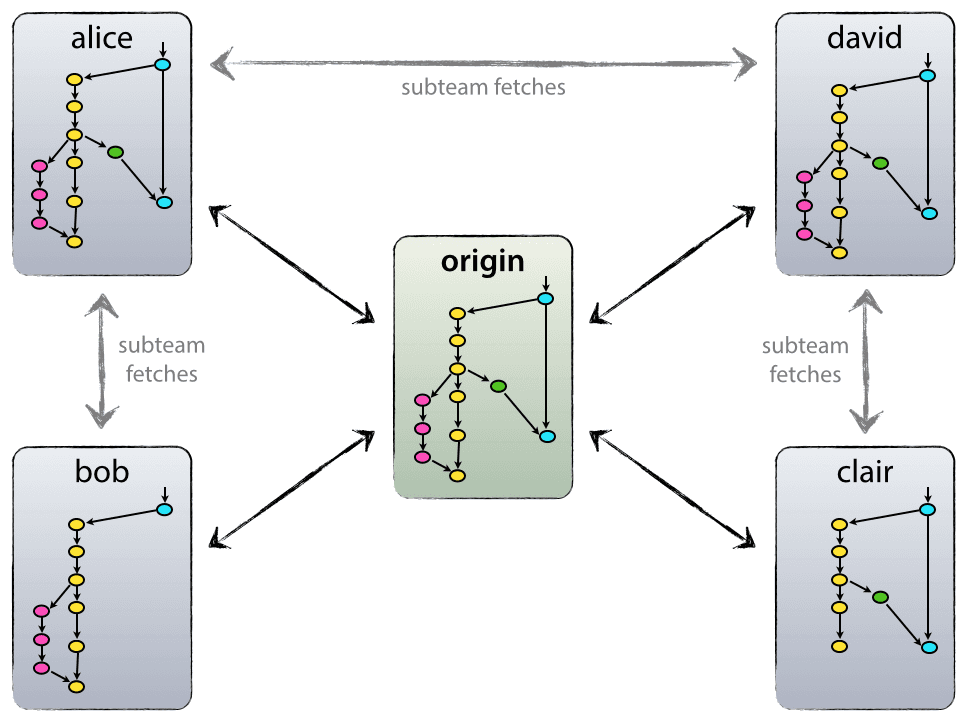
\includegraphics[max width=7cm, max height=5.6cm]{Kapitel/TechnischeGrundlagen/Bilder/gitbranching2.png}
				\vspace{0.1cm}
				\captionof{figure}{Teamarbeit mit mehreren remotes \cite{gitbranching}}
			\end{center}
		\end{mdframed}
	\end{textblock}
    \only<2->{
		\begin{textblock}{7.6}(8,3.1)
			\begin{mdframed}[backgroundcolor=white]
				\begin{center}
					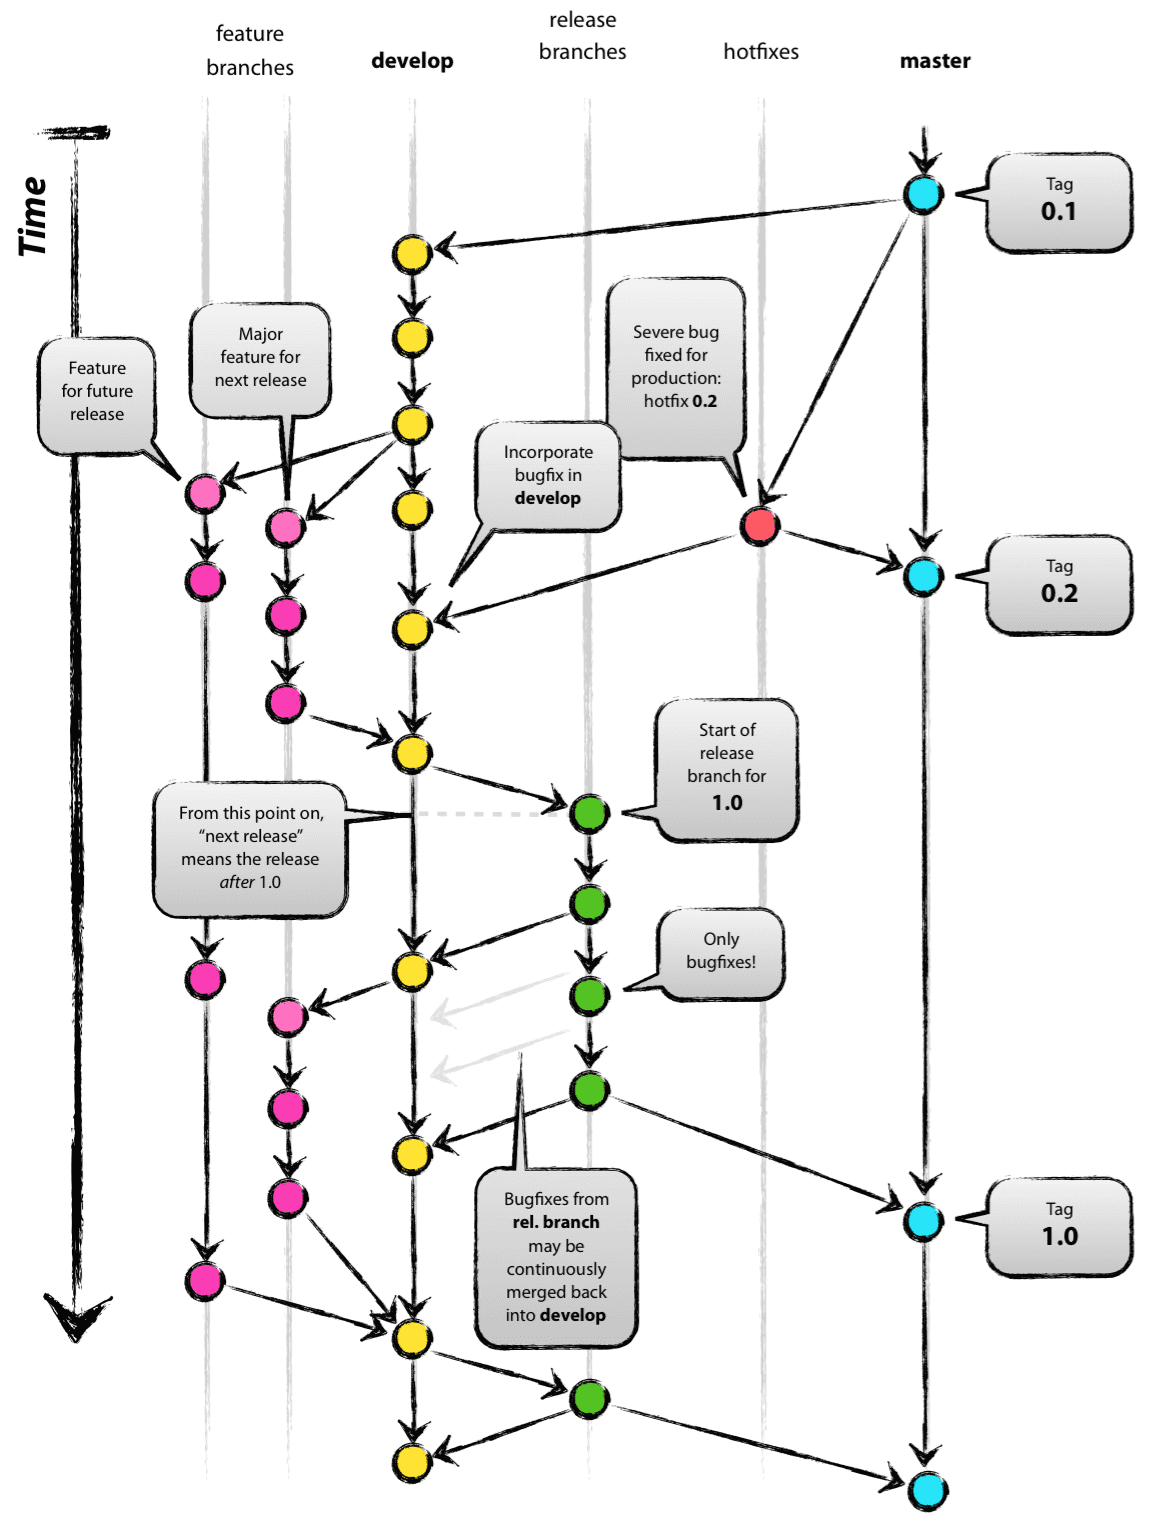
\includegraphics[max width=7cm, max height=5.6cm]{Kapitel/TechnischeGrundlagen/Bilder/gitbranching.png}
					\vspace{0.2cm}
					\captionof{figure}{Komplexe branching-Strategie \cite{gitbranching}}
				\end{center}
			\end{mdframed}
		\end{textblock}
    }
\end{frame}

\begin{frame}{Übung: git}
    \note{
        \begin{itemize}
            \item Gitlab: Open Source (inhouse betreibbar), kostenfreie private Repositories, einfach konfigurierbares CI/CD. Aber grundsätzlich: Geschmackssache.
	    \item Aktuelle Nachrichten?
            \item<3-> Branch-Anpassung
            \item<5-> Abfrage: Ist .git-credentials ein Problem? Hinweisen auf häufige Wiederverwendung von Mail-Passwort-Kombinationen
            \item<7-> \textbf{Diskutieren}: Passwort für key. Ist passwortloser key besser oder schlechter als .git-credentials? Hinweis auf keepass
            \item<8-> \textbf{Diskutieren}: Ist git push --force nach reset auf gepushten commit  eine gute Idee?
        \end{itemize}
    }
    \begin{itemize}
        \item Erstellung eines gitlab-Accounts
        \item<2-> Neues Projekt erstellen, README anpassen (online)
        \item<3-> clone, README anpassen, commit
        \item<4-> push... Aber wo geht es hin? git remote! Und was geht da hin? git branch
        \item<5-> Credentials merken...
        \item<6-> ...und gleich wieder löschen! 
        \item<7-> Alternative: \href{https://docs.gitlab.com/ee/ssh/}{SSH-Key}. Dafür: clone über SSH (oder remote anpassen?)
        \item<8-> Fehler rückgängig machen: git reset (vor und nach push)
    \end{itemize}
\end{frame}

\begin{frame}{Exkurs: Warum Python?}
    \note{
        \only<1-2>{
		   \begin{itemize}
			   \item Java super für portable, performante Applikationen, aber mies für Prototyping
			   \item Python super für Prototyping, aber schlecht für Stabilität
			   \item PHP Totalausfall bei Wartbarkeit+Sicherheit, aber toll für schnelle kleine Webapp
			   \item Wünsche JavaScript schnellen und schmerzhaften Tod, setze es trotzdem für interaktive Visualisierungen ein
		   \end{itemize}
        }
        \only<3->{
            Mini-Whiteboard: Was ist wichtig bei der Entscheidung für eine Sprache für ein Projekt?
            \textbf{Zeit: 5 Minuten}
            \begin{itemize}
                \item Entwickler: Einer? Mehrere? Community oder Spaltungen? Aktivität der Entwicklung? (wikipedia, PEPs, BDFL)
                \item Anzahl an reifen Projekten in Sprache (z.B. Betriebssysteme)
                \item Bekannte Schwachstellen und Reaktionen (exploit-db.com, cve.mitre.org etc), konkretes Beispiel: www.cvedetails.com, Oracle (Page 10), Java, Metasploit modules, CVE-2012-4681 Java 7 Applet Remote Code Execution. Google: Page 12.
                \item Geeignetheit der Features für Problem (bsp. R, shell, PHP)
                \item Verfügbarkeit von relevanten Bibliotheken (pypi.org)
		\item Verfügbarkeit aktueller Entwicklungstools (Spyder, PyCharm)
                \item Lizenz: Vorhanden? Falls ja, Bedingungen, bsp. GPL vs. LGPL. Python: PSF 
            \end{itemize}
        }
    }
    Wichtig in Programmierung: Weniger eine konkrete Sprache, mehr breites Wissen und Verständnis von Konzepten. Also: Richtige Programmiersprache für das Problem wählen! \only<2->{
        Aber: Was heißt ``richtig?''
    }
    \only<4->{
        \textbf{ Und ist Python ``richtig''?}
    }
    \only<3->{
        \begin{itemize}
            \item[\only<4>{\textbullet}\only<5->{\checkmark}] Aktive Entwicklung
            \item[\only<4-5>{\textbullet}\only<6->{\checkmark}] Starke Aktuere in der Community
            \item[\only<4-6>{\textbullet}\only<7->{\checkmark}] Vorhandensein reifer Produkte
            \item[\only<4-7>{\textbullet}\only<8->{\checkmark}] Sicherheit
            \item[\only<4-8>{\textbullet}\only<9->{\checkmark}] Relevante Bibliotheken und Entwicklungstools
            \item[\only<4-9>{\textbullet}\only<10->{\checkmark}] Bekannte und nutzbare Lizenz
            \item[\only<4-10>{\textbullet}\only<11->{?}] Ausreichende ROI bei fehlenden Vorkenntnissen
        \end{itemize}
    }
\end{frame}

\begin{frame}{Exkurs: Warum Python: ROI}
  \only<2->{Was sind typische Aufgabenbereiche für Bioinformatiker?\vspace{0.3cm}}
  \note<2>{
   Vorsicht:
   \begin{itemize}
       \item Das bezieht sich alles primär auf Bioinformatik
       \item Medizininformatik: 99\% Windows
   \end{itemize}
  }
  \begin{columns}
   \begin{column}{0.5\textwidth}
     \only<3->{\centering \textbf{Softwareentwicklung}}
     \begin{itemize}
       \item<3->Produktzentriert
       \item<3->Performante Implementation eines Algorithmus
       \item<3->Stabilität, Reproduzierbarkeit, gutes User Interface
       \item<4->Primär Java, C++
     \end{itemize}
   \end{column}
   \begin{column}{0.5\textwidth}
     \only<5->{\centering \textbf{Datenauswertung}}
     \begin{itemize}
       \item<5->Projektzentriert
       \item<5->Verwendung existierender Tools
       \item<5->Entwicklung von Pipelines
       \item<5->Implementation kleinerer Algorithmen
       \item<5->Flexibilität, bedarfsgerechte Visualisierung
       \item<6->Primär Python, R
     \end{itemize}
   \end{column}
  \end{columns}
\end{frame}

\begin{frame}{Exkurs: Warum Python: ROI II}
  \begin{textblock}{10}(1,2.8)
   \begin{figure}[h!]
     \frame{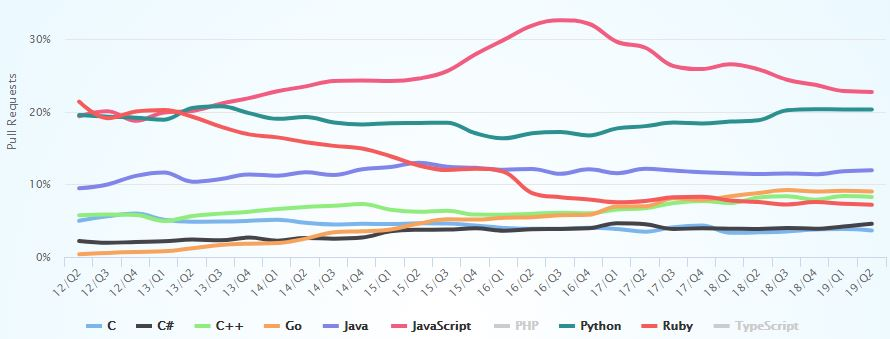
\includegraphics[width=12cm]{Kapitel/TechnischeGrundlagen/Bilder/PythonPulls.jpg}}
     \vspace{0cm}
     \caption{Pull-requests auf github nach Sprache \cite{PythonPulls}}
   \end{figure}
  \end{textblock}
 \only<2->{
  \begin{textblock}{10}(0.9,3)
   \begin{figure}[h!]
     \frame{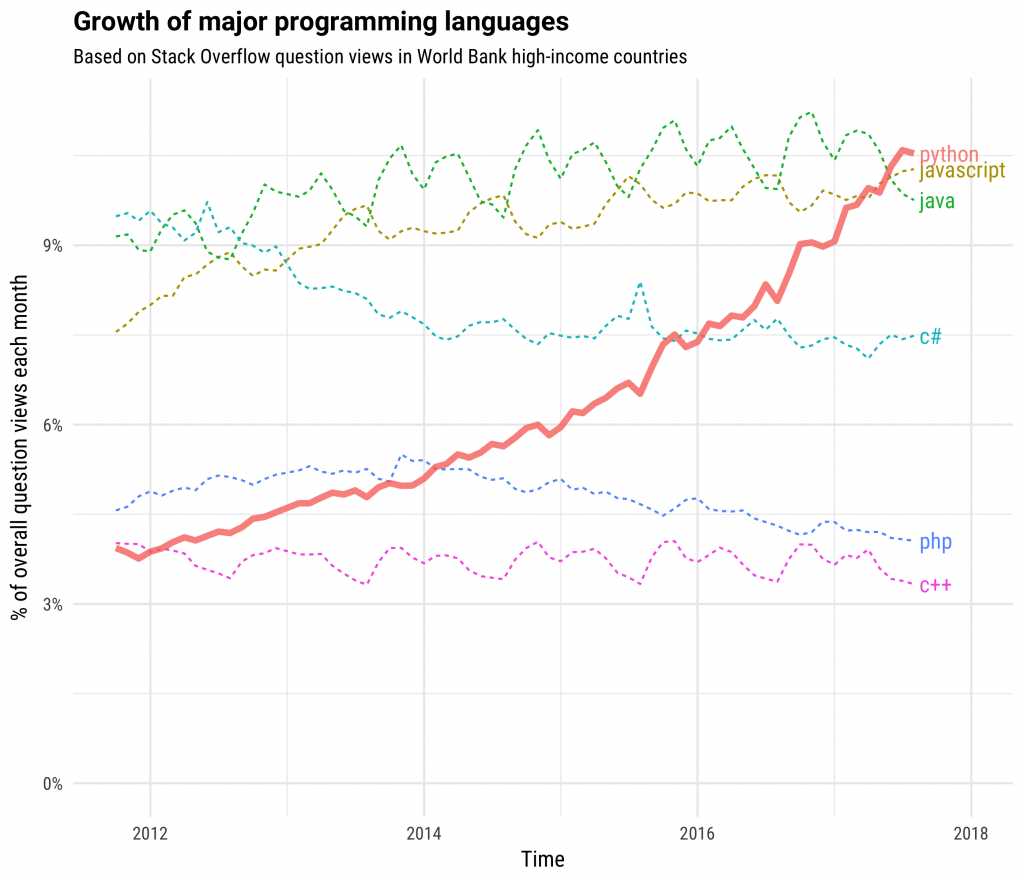
\includegraphics[width=6.5cm]{Kapitel/TechnischeGrundlagen/Bilder/PythonQuestions.png}}
     \vspace{0.3cm}
     \caption{Fragen auf StackOverflow nach Sprache \cite{PythonQuestions}}
   \end{figure}
  \end{textblock}
 }
 \only<3->{
  \begin{textblock}{10}(7.1,0.6)
   \begin{figure}[h!]
     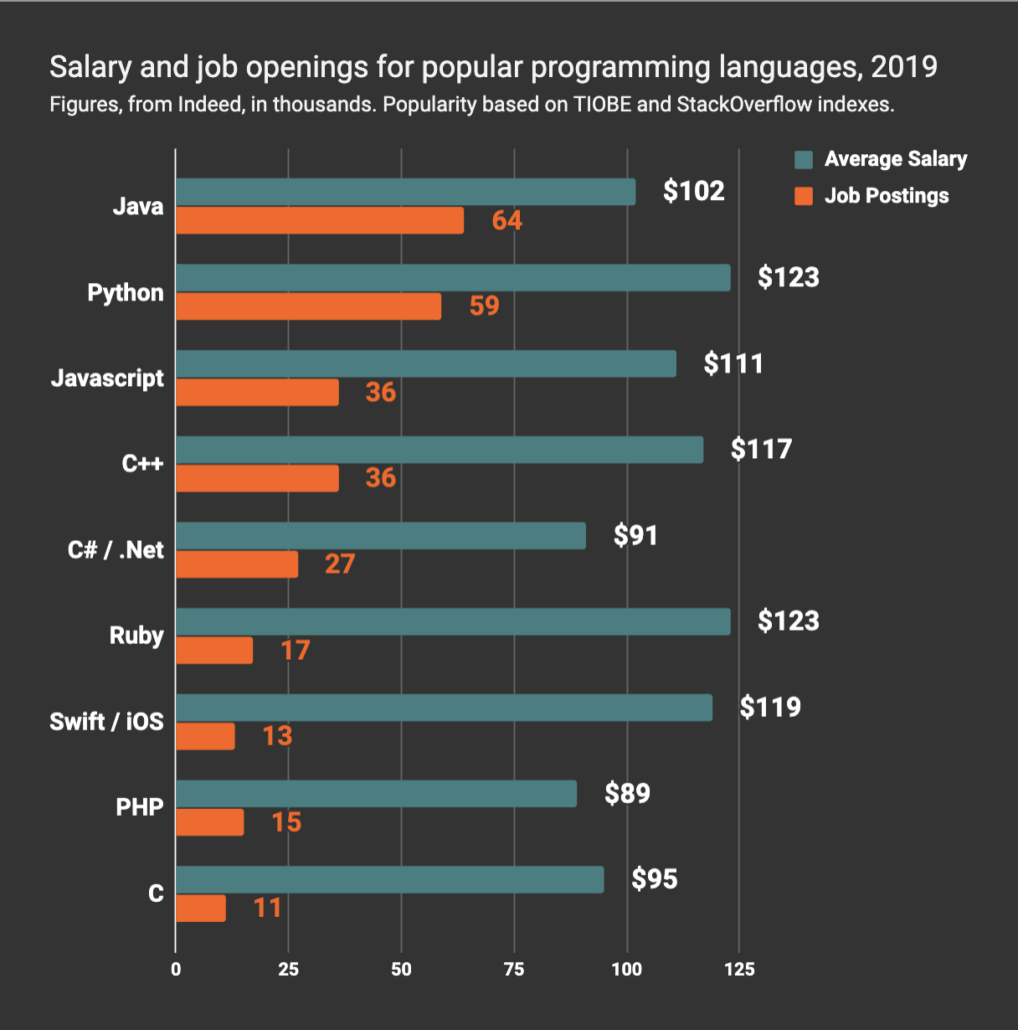
\includegraphics[width=7cm]{Kapitel/TechnischeGrundlagen/Bilder/LanguagesSalary.png}
     \vspace{0.3cm}
     \caption{Einkommen und Stellen nach Programmiersprache \cite{LanguagesSalary}}
   \end{figure}
  \end{textblock}
 } 
\end{frame}



\begin{frame}[fragile]{\only<1-4,6->{Python}}
    \note{
        \begin{itemize}
            \item Unterschiede compiliert and linked, interpretiert (bytecode), JIT
            \item Source code $\rightarrow$ Object code $\rightarrow$ Executable
        \end{itemize}
    }
    \begin{itemize}
        \item Interpretierte Sprache
        \item<4-> Multi-paradigm: Objektorientiert, mit funktionalen Elementen
        \item<4-> Typisierung: Dynamisch, stark (dynamically, strongly typed)
        \item<6-> Automatisches Speichermanagement
        \item<7-> Designziel: Einfach zu lesen und zu schreiben, prägnant (wenig boilerplate code)
        \item<7-> Einrückung statt Klammern
    \end{itemize}
    \only<2>{
        \begin{textblock}{10}(3,0.2)
            \begin{figure}[h!]
                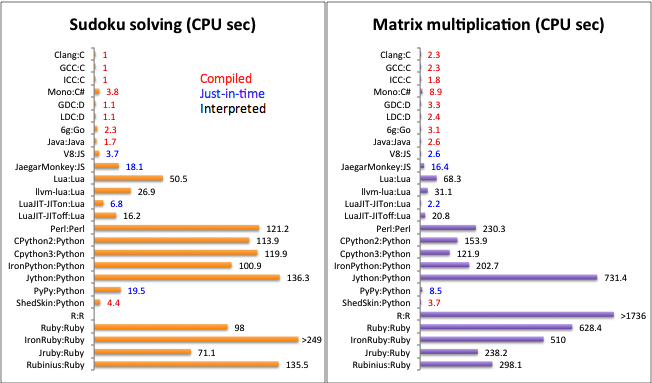
\includegraphics[height=7.3cm, left]{Kapitel/TechnischeGrundlagen/Bilder/langperformance.png}
				\vspace{0cm}
                \caption{Beispielhafter Performance-Vergleich zwischen Sprachen \cite{langperformance}}
            \end{figure}
        \end{textblock}
    }
    \only<3> {
        \begin{textblock}{10}(2,4)
            \begin{figure}
                \lstinputlisting[frame=single, language=Python, backgroundcolor = \color{white}]{Uebungen/hello.py}
                \caption{Beispiel für Laufzeitfehler}
            \end{figure}
        \end{textblock}    
    }
    \only<5> {
        \begin{figure}
            \begin{textblock}{14}(1,0.5)
                \lstinputlisting[frame=single, language=Python, backgroundcolor = \color{white}]{Uebungen/types.py}
            \end{textblock}    
            \begin{textblock}{14}(1,5.5)
                \lstinputlisting[frame=single, language=Java, backgroundcolor = \color{white}]{Uebungen/types.java}
                \caption{Java und Python: Schwache und starke Typisierung}
            \end{textblock}    
        \end{figure}
    }
\end{frame}
